% === Cours de Java
% === Chapitre : Introduction

\subsection{La machine virtuelle}

\begin{frame}
	\begin{center}
		Java est \emph{compil�} puis \emph{interpr�t�}.
	\par
	L'interpr�teur Java est la machine virtuelle (\sigle{JVM})
	\par
	Le langage de bas niveau interpr�t� par la \sigle{JVM} est le \emph{\sigle{bytecode}}
\end{center}
\end{frame}

\begin{frame}{La machine virtuelle}
\begin{center}
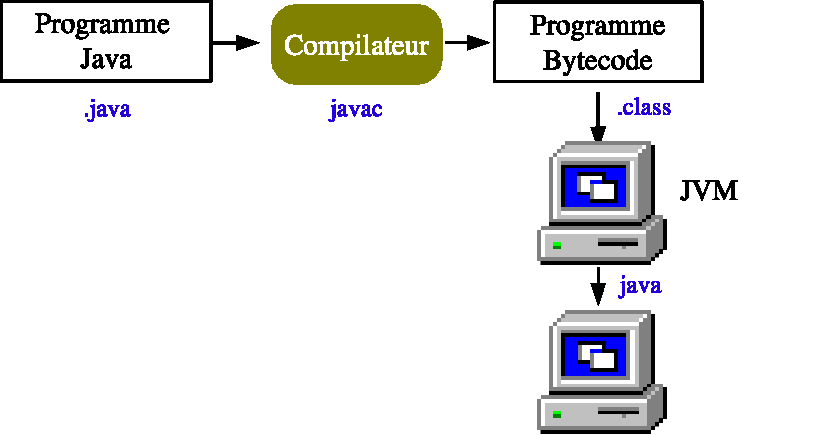
\includegraphics[scale=0.8]{../img/java-jvm-jvm2} 
\end{center}
\end{frame}

\imgfullh{../img/Sun_and_rain_by_emolawn.jpg}
{\begin{flushright}\large\bf\color{ghostwhite} Avantages et\\inconv�nients\end{flushright}}
	{http://emolawn.deviantart.com/art/Sun-and-rain-85676638}
\note[item]{Java serait lent � interpr�ter (langage haut niveau).  Donc, introduction d'un niveau interm�diaire, le Bytecode, qui est
 proche d'un langage d'assemblage, 
 plus rapide � interpr�ter.
C'est en fait le langage de la JVM}


\begin{frame}[fragile]{Exemple: premier programme}
Prenons un exemple \textit{(fichier \code{Hello.java})}
\begin{Java}
// Mon premier programme
public class Hello {
  public static void main(String[] args) {
    System.out.println("Bonjour !");
  }
}
\end{Java}
Compilons-le \texttt{\$ javac Hello.java}
\par
On obtient la version compil�e, le \sigle{bytecode} (\code|Hello.class|)
\par
On peut l'ex�cuter \texttt{\$ java Hello}\\
\texttt{Bonjour !}
\end{frame}

\subsection{Les outils de d�veloppement}

\imgfullh{../img/righttool-3348965007_b3049c78fe_b.jpg}
{\vspace{-1cm}\color{cadetgrey}\Large\bf Fourbir ses armes}
{https://www.flickr.com/photos/ebarney/3348965007/in/photostream/}


\begin{frame}{Les outils de d�veloppement}
Les �ditions de \sigle{Java}
\begin{itemize}
	\item \emph{Java SE} (�dition standard)
	\item \emph{Java ME} (�dition mobile - plus l�ger) 
	\item \emph{Java EE} (�dition entreprise - plus complet)
\end{itemize}
\begin{wrapfigure}{r}{17mm}
	
\includegraphics[width=17mm]{../img/java-download.png}
\end{wrapfigure}
\bigskip
O� trouver \code|javac| et \code|java| ?
\par
\emph{\sigle{JRE}} (\textit{Java Runtime Environment}) \\
\emph{\sigle{JDK}} (\textit{Java Development Kit})
\end{frame}


\full[bluepigment]{
	\begin{center}
		\Large\bf\color{azuremist}
		�diter \\ Compiler \\ Ex�cuter
	\end{center}
}

\begin{frame}{Les outils de d�veloppement}
 \par{\bf\Huge 1} 
\begin{itemize}
\item Un \emph{�diteur avec coloration syntaxique}:
	\emph{\sigle{gVim}}, \emph{\sigle{Notepad++}}, \emph{\sigle{nano}}, \dots
\item Gestion manuelle des noms et emplacements des fichiers
\item Compilation et ex�cution en ligne de commande
\end{itemize}
\end{frame}

\begin{frame}{Les outils de d�veloppement}
 \par{\bf\Huge 2}
 \begin{itemize}
	\item Un \textit{\emph{E}nvironnement de \emph{D}�veloppement \emph{I}nt�gr�} : 
	\emph{\sigle{Netbeans}}, \emph{\sigle{Eclipse}}, \dots
  	\item Int�gre tout le processus de d�veloppement  
  \end{itemize}
\end{frame}


